\documentclass[a4paper,12pt]{article}
\usepackage[utf8]{inputenc}
\usepackage[spanish]{babel}
\usepackage{color}
\usepackage{parskip}
\usepackage{graphicx}
\usepackage{multirow}
\usepackage{listings}
\usepackage{vmargin}
\graphicspath{ {imagenes/} }
\definecolor{mygreen}{rgb}{0,0.6,0}
\definecolor{lbcolor}{rgb}{0.9,0.9,0.9}
\usepackage{epstopdf}


\setpapersize{A4}
\setmargins{2.5cm}       % margen izquierdo
{1.5cm}                        % margen superior
{16.5cm}                      % anchura del texto
{23.42cm}                    % altura del texto
{10pt}                           % altura de los encabezados
{1cm}                           % espacio entre el texto y los encabezados
{0pt}                             % altura del pie de página
{2cm}     

\lstset{
    tabsize=4,    
%   rulecolor=,
    language=[GNU]C++,
        basicstyle=\tiny,
        aboveskip={1.5\baselineskip},
        columns=fixed,
        showstringspaces=false,
        extendedchars=false,
        breaklines=true,
        prebreak = \raisebox{0ex}[0ex][0ex]{\ensuremath{\hookleftarrow}},
        frame=single,
        showtabs=false,
        showspaces=false,
        showstringspaces=false,
        identifierstyle=\ttfamily,
        keywordstyle=\color[rgb]{0,0,1},
        commentstyle=\color[rgb]{0.026,0.112,0.095},
        stringstyle=\color{red},
        numberstyle=\color[rgb]{0.205, 0.142, 0.73},
%        \lstdefinestyle{C++}{language=C++,style=numbers}’.
}

\begin{document}
\begin{titlepage}

\begin{center}
\vspace*{-1in}

\begin{large}
UNIVERSIDAD NACIONAL DE SAN AGUSTÍN\\
\vspace*{0.15in}
ESCUELA PROFESIONAL DE CIENCIA DE LA COMPUTACIÓN\\
\end{large}
\begin{figure}[htb]
\centering

\includegraphics[scale=0.13]{/home/xnpio/Documentos/Caratula/logo.eps}
\end{figure}
\vspace*{0.15in}
\begin{large}
TEMA:\\
\end{large}
\vspace*{0.2in}
\begin{Large}
\textbf{} \\
\end{Large}
\vspace{8mm}

\begin{large}
Curso:\\
\end{large}
\vspace*{0.2in}
\begin{Large}
\textbf{MATEMÁTICA APLICADA A LA COMPUTACIÓN} \\
\end{Large}

\vspace{8mm}

\begin{large}
\textbf{Presentado por:}\\

\begin{flushleft}

\hspace{7cm} Christofer Chávez Carazas \\

\end{flushleft}
\end{large}
\vspace{4cm}
\rule{80mm}{0.1mm}\\
\vspace*{0.1in}

\begin{large}
Arequipa - Perú \\
2017 \\
\end{large}
\end{center}
\end{titlepage}

\begin{Large}
 NOMBRE $->$ CHRISTOFER FABIÁN CHÁVEZ CARAZAS
\end{Large}

 \section{Código}
 
 \begin{lstlisting}
#include <iostream>
#include <cmath>
#include "OperacionesMatriz.h"

using namespace std;

Num buscarMayor(Lista & b){
	Num res = -1;
	for(auto iter = b.begin(); iter != b.end(); iter++){
		if(abs(*iter) > res or res == -1) res = abs(*iter);
	}
	return res;
}

void MetodoPotencias(int iteraciones, Matriz & m, Lista ini){
	Lista u;
	Lista v = ini;
	for(int i = 0; i < iteraciones; i++){
		u = m * v;
		Num dominante = buscarMayor(u);
		v = u * (1.0 / dominante);
		cout<<"------U_"<<i+1<<"------"<<endl;
		mostrarLista(u);
		cout<<"------V_"<<i+1<<"------"<<endl;
		mostrarLista(v);
	}
}

int main(int argc, char * argv[]){
	if(argc != 2){
		cout<<"Faltan argumentos: <numIteraciones>"<<endl;
		return 0;
	}
	string temp(argv[1]);
	int it = stoi(temp);
	Matriz m = {{3,-1,0},{-1,2,-1},{0,-1,3}};
	Lista ini = {1,1,1};
	MetodoPotencias(it,m,ini);
}
 \end{lstlisting}

\section{Resultados}

\begin{figure}[h]
  \centering
  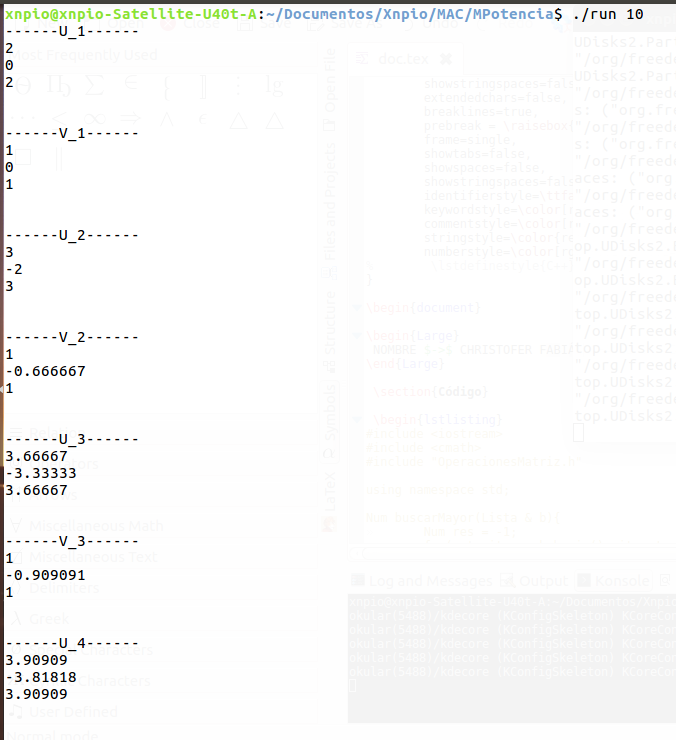
\includegraphics[scale = 0.25]{1.png}
\end{figure}

\begin{figure}[h]
  \centering
  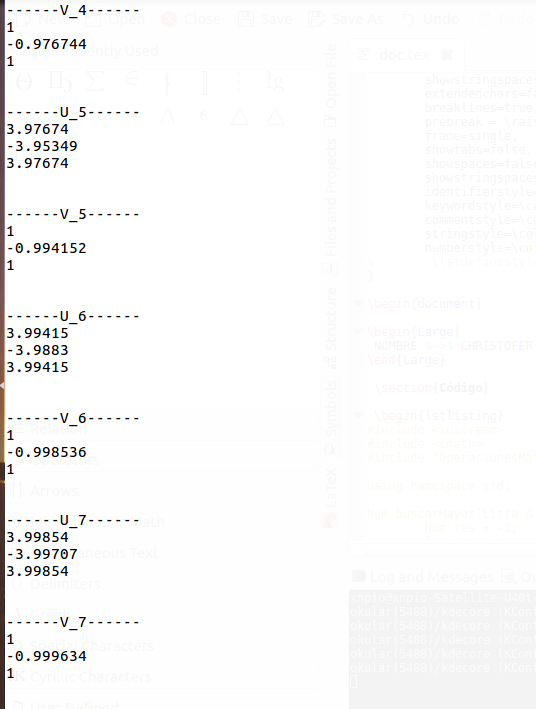
\includegraphics[scale = 0.4]{2.png}
\end{figure}

\begin{figure}[h]
  \centering
  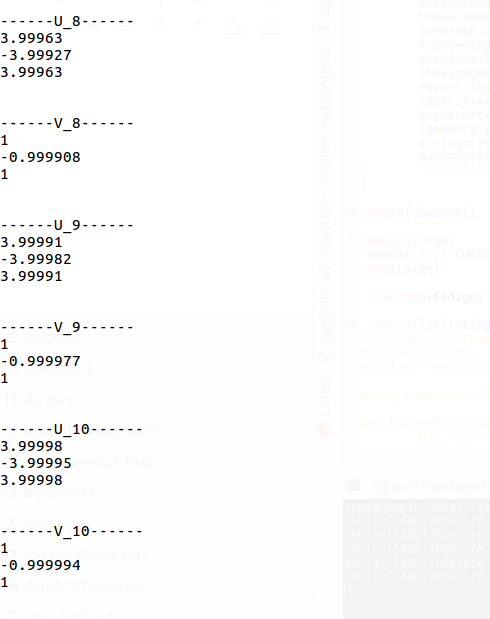
\includegraphics[scale = 0.4]{3.png}
\end{figure}


\end{document}
